
\section{Empirical Validation}
\label{sec:results}

To validate the performance of our method, we test our framework across multiple classification datasets. Our networks are composed of a 1-Lipschitz feature extractor followed by a classification layer that ensures that every output respects a $1$-Lipschitz condition. 
We provide information about of the computational overhead of training Lipschitz-constrained networks and the model architectures used for other methods in Appendix~\ref{app:models_experiments}. Finally, our code will be made available on the following \href{https://github.com/deel-ai-papers/lip-rcp}{github} repository.


\paragraph{Training scheme} We leverage networks with Lipschitz and orthogonality constraints from the library introduced in \citet{boissin2025adaptiveorthogonalconvolutionscheme} to balance both performance and minimal training overhead. More details are provided in Appendix~\ref{app:experimental_settings}. 

\begin{figure*}[!t]
    \centering
    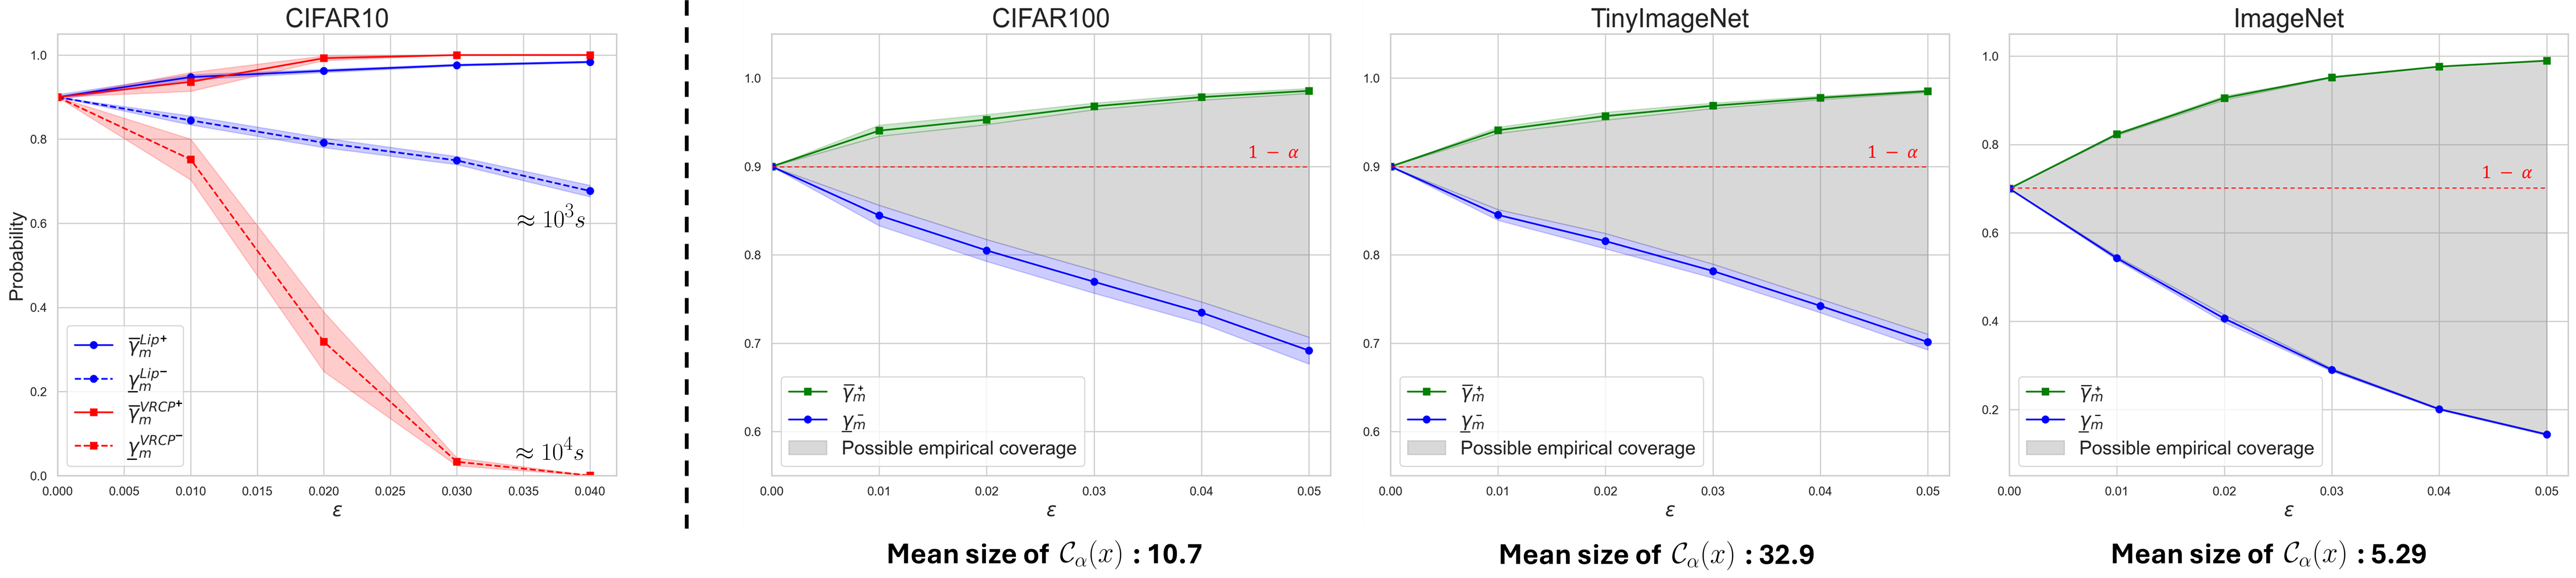
\includegraphics[width=\linewidth]{banner_coverage_speed.png}
    \caption{(Left): Comparison between vanilla CP coverage bounds using Lipschitz bounds or the \emph{CROWN} method with $\delta = 10^{-4}$. Approximate  computation times are also provided. (Right): Corrected $\covmaxmp$ and $\covminmm$ bounds for vanilla CP methods under $\epsilon$ bounded adversarial noise computed on 1-Lipschitz networks given $\delta = 10^{-4}$. Mean prediction set size on clean data is indicated below each plot. We take $n_{cal}=15000$ and $n_{eval}=35000$ for ImageNet.}
    \label{fig:coverage}
\end{figure*}
 
\subsection{Robust CP Comparison}
\label{sec:resultsclassic}

We evaluate our method on the \textsl{CIFAR-10}, \textsl{CIFAR-100} and \textsl{TinyImageNet} datasets. Our methodology follows that of the benchmark of \emph{VRCP} and we adopt the same calibration, holdout and test set sizes as \citet{vrcp} on all these datasets. Also, we give the mean values of the robust CP set sizes and the conformal coverage of these robust sets across $25$ different random samplings of $\CalDataset$ and $\TestDataset$ (as well as $\mathcal{D}_\mathrm{holdout}$ for \emph{PTT}) that were unseen during training. We report our results in Fig.~\ref{fig:fastcp_results} where we also plot the measurements made by \citet{vrcp} with different markers. To allow fair comparison with verification methods, we train specific neural networks for \emph{VRCP} on the \textsl{CIFAR-10} dataset according to Appendix B of the associated paper. This allows the \emph{CROWN}~\cite{zhang2018efficientneuralnetworkrobustness} method to run efficiently on this model. For \emph{CAS}, we use ResNet50 networks. Finally, we do not benchmark the \emph{PRCP} method whose robustness guarantees are specific to the type of adversarial perturbation.

\paragraph{Interpretation} Our method outperforms existing robust CP approaches across all tested datasets, Fig.~\ref{fig:fastcp_results}, it provides smaller robust CP sets while maintaining conformal coverage close to $1-\alpha$. We give the following explanations to these results. First, the Lipschitz-constrained model training approach we use is more efficient at promoting robustness. Also, neural networks with orthogonality constraints allow tight estimations of their conservative scores. Additionally, smoothing methods suffer from finite sample MC estimations in more than one way: as both a corrective factor is added to the smoothed scores, and the error probability of the MC estimation also necessitates adjusting the quantile computation. Finally, smoothing methods require an unrealistic number of MC samplings to obtain meaningful sets.

\paragraph{Scaling to the ImageNet dataset} In order to evaluate the scalability of our method, we also validate it on the \textsl{ImageNet} dataset. Given the poor scalability of formal verification methods, we were not able to apply \emph{VRCP} on the \textsl{ImageNet} dataset. 
We therefore compare our method to \emph{CAS} on a ResNet50 network, being generally the best performing competing approach. %\emph{RSCP}.
 Our model is described in Appendix~\ref{app:model_implementation}. 

Finally, we used a restricted set of $n=500$ data points to evaluate the \emph{CAS} method as done in \citet{cas}, given its intensive computational budget.  
For both methods we use $40\%$ of the data points for calibration and the rest for testing. The obtained results are given in Table~\ref{tab:imagenet}. 

\begin{table}[h]
  \centering
  \sisetup{
    detect-weight = true,
    detect-family = true,
    table-number-alignment = center
  }
  \begin{tabular}{
    l
    S[table-format=4.1]
    S[table-format=3.1]
    l
    S[table-format=1.3]
  }
    \toprule
    \textbf{Method}   & {\textbf{Set size}} & {\textbf{Cov. (\%)}} & {\textbf{\(n\)}} & {\textbf{Time (s)}} \\
    \midrule
    \emph{CAS}        & 1000.0               & 100.0                    & $5\cdot10^2$     & 7.920                        \\
    \emph{lip-rcp}    & \bfseries 111.0      & \bfseries 97.4           & $5\cdot10^4$     & 0.012                        \\
    \bottomrule
  \end{tabular}
  \caption{Robust CP set sizes and empirical test coverage at \(\epsilon=0.02\), \(\alpha=0.1\) on ImageNet (using \emph{CAS} with \(n_{\mathrm{mc}}=1024\)). One additional run of our method at \(n=5\cdot10^2\) yielded a set size of 118.5 and 97.5\% coverage. The time is given \textit{per sample}.}
  \label{tab:imagenet}
\end{table}

\subsection{Certifiable Vanilla CP Coverage Bounds Results}
\label{sec:resultscoverage}

In this section, we compute respectively lower and upper bounds of \(\covminmm\) and \(\covmaxmp\) introduced in Section~\ref{sec:vanillacoverage} by both Lipschitz and formal verification methods.
We first perform vanilla split CP on \(\CalDataset\) consisting of \(n_{cal} = 3000\) samples. Next, we compute empirical approximations \(\covmaxm\) and \(\covminm\) as in \eqref{eq:covmaxm} and \eqref{eq:covminm} on an evaluation dataset \(\HoldoutDataset\) with \(n_{eval} = 5000\) samples with both Lipschitz bounds and the \emph{CROWN} formal verification method.
%extended to our theoretical framework. 
We then compute the corrected estimates  \(\covmaxmp\) and \(\covminmm\) as in \eqref{eq:covmaxmp} and \eqref{eq:covminmm} guaranteed in Theorem~\ref{thm:robustcoverageuniform} by binary search.
We repeat this process over 20 randomly sampled, non-overlapping pairs of \(\CalDataset\) and \(\HoldoutDataset\), and plot the mean value with an uncertainty band of 1 standard deviation.
The resulting coverage metrics are shown on Fig.~\ref{fig:coverage} (left) on the \textsl{CIFAR-10} dataset for both computation methods with their associated models.

We further compute the worst-case conformal coverage values of standard conformal prediction (CP) sets under \(\epsilon\)-bounded perturbations across all previously mentioned datasets. Due to the larger scale of these tasks, we are only able to compute the bounds for $1$-Lipschitz models. The results are presented in Fig.~\ref{fig:coverage} (right).

\paragraph{Interpretation} As illustrated in Fig.~\ref{fig:coverage} (left), Lipschitz-constrained models yield less pessimistic bounds than verification for the worst-case coverage of vanilla CP under \(\epsilon\)-bounded adversarial perturbations. This can be explained by the limited scalability of formal verification methods to larger neural networks. Also, Fig~\ref{fig:coverage} (right) uncovers how providing coverage bounds for CP methods applied to robust networks conserves the small and informative nature of CP sets while providing error guarantees under bounded attacks.